\section{Formulation and Overall flow}
\begin{figure}[!htb]
\centering
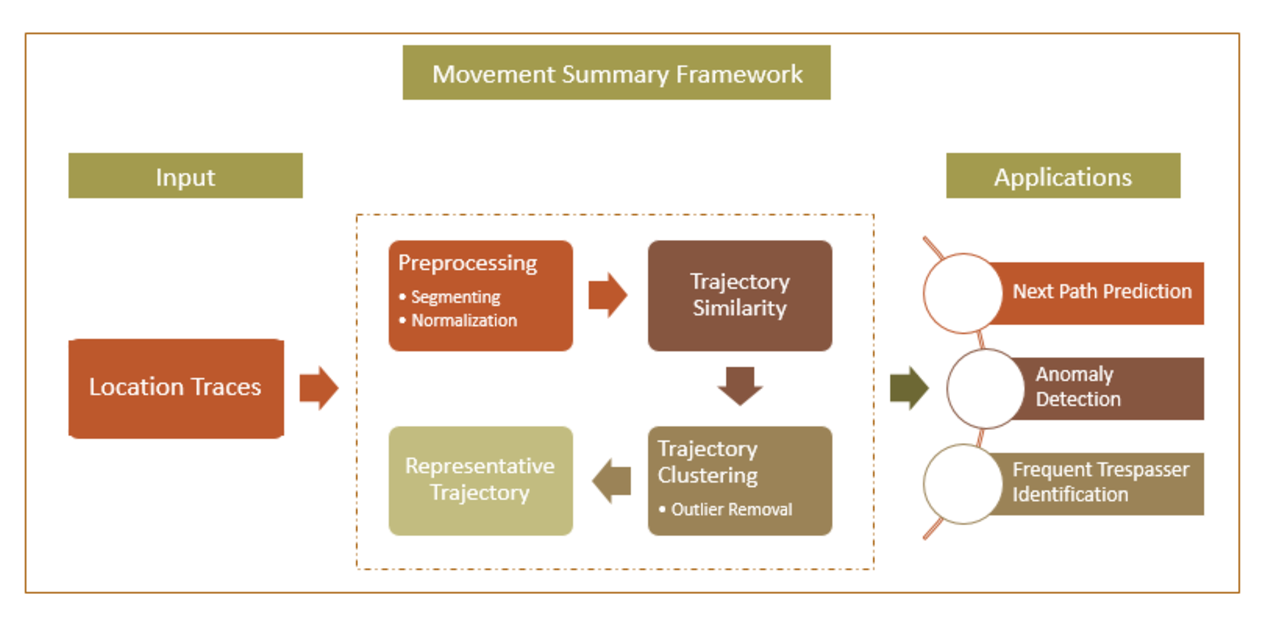
\includegraphics[scale=0.6]{figs/overallflow.eps}
\caption{Overall Flow}
\label{fig:components}
\end{figure}

Figure \ref{fig:components} provides the different components for computing the Mobility Summary, which in turn can be used a variety of applications that rely on frequent-mobility based queries.The various components of the flow are described briefly below: 

%% 1 Trajectory Segmentation
%% 2. Trajectory Similarity
%% 3. Clustering
%% 
\paragraph{Input}
The input in the form of a raw collection of three tuples, which are the location traces of the person or user.
\paragraph{Preprocessing}
Pre-processing consists of the steps segmenting which is the process of making meaningful trips out of the raw traces. The second component is normalization.
\paragraph{Trajectory Similarity} 
This is the module which defines and computes the similarity between all the pairs of trajectories in the dataset. This is a very crucial step as the clustering depends on the goodness of the similarity measure.
\paragraph{Trajectory Clustering}
This module takes as input the similarity matrix formed in the earlier step, and runs a clustering algorithm on it and outputs a final cluster of trajectories. This step also encompasses outlier or anomaly detection.
\paragraph{Representative Trajectory} 
Once we have all the final clusters, we have to come up with on trajectory per cluster which can act as the representative trajectory for that cluster. This task is taken up in this section.
\paragraph{Applications}
The applications of Movement Summary include next path prediction and anomaly detection.
 
